\graphicspath{{litreview/fig/}}

\chapter{Literature Review}
\label{chap:litreview}


\section{Theory and applications of superconductivity}
In order to understand and apply the methods described in \cite{fluxNoiseSquidsStevenAnton} one must first understand the basic theory behind superconductivity as well as some examples of how this theory is used in practice.

\subsection{Superconductivity}
\textcolor{red}{REVIEW NEEDED}

Since the first discovery of superconductivity a couple of successfully theories have been put forth to explain the phenomenon. The London theory is a framework that describes the qualitative behaviour of superconductors and correctly describes perfect diamagnetic and zero resistance but fails to explain the effect on a microscopic level \cite{Golubov_1998}. The London equations (equation \ref{london1} and equation \ref{london2}) \cite{Tinkham_2015} is an addition to Maxwell's equations.
\begin{equation}
    E = \frac{\partial}{\partial t}(\Lambda J_s)
    \label{london1}
\end{equation}
\begin{equation}
    h = -c \nabla\times (\Lambda J_s)
    \label{london2}
\end{equation}
Here $\Lambda$ is a phenomenological parameter determined through experimentation. The London equations allow us to calculate the current distribution in a superconductor which is very important to the objective of this project. BCS theory put forth a microscopic model of superconductors and explains the phenomenon as a quantum mechanical effect. The details are out of scope for this project but on a crude qualitative level BCS theory can be explained by the pairing of electrons in the crystal lattice of the superconductor allowing them to be considered one particle. These particles are known as cooper-pairs. At extremely low temperatures the formation of these cooper pairs are energetically favourable \cite{Feynman_Leighton_Sands_2013}. Electron pairs in this state can flow through the superconductor unimpeded. BCS theory is the most successful model of superconductivity discovered to date. 

\subsection{The Josephson junction}
In superconducting electronics the active component is the Josephson junction \cite{Duzer_1999_Princip_Super}. The Josephson junction refers to a situation where two superconductors are connected through a thin non-conductive barrier. If this barrier is thin enough one can observe what is known as the Josephson effect. This phenomena is can be explained by considering the effect of quantum tunnelling of cooper pairs through the non-conductive boundary. For a sufficiently large barrier one can express the ensemble average wave function in each superconductor independently\cite{Duzer_1999_Princip_Super}:
\begin{equation}
    \Psi = |\Psi(\Vec{r})| \exp{\{i\theta(\Vec{r})\}}
    \label{eq:ensembleWave}
\end{equation}
This is due to the fact that it is energetically favourable for cooper pairs in proximity to one another to lock phases \cite{Duzer_1999_Princip_Super} allowing one to express a large collection of these cooper pairs as one ensemble wave function. The idea that it is energetically favourable for cooper-pairs in proximity to one another extends to the situation where the superconductors are separated by an insulating boundary. When the barrier is sufficiently small the energy of the system can be reduced by the coupling of wave functions in their respective superconductors \cite{Duzer_1999_Princip_Super}. This results in cooper-pairs being able to move across the boundary without energy loss. Following the derivation in \cite{Feynman_Leighton_Sands_2013} one can describe the system behaviour using Schrödinger's equation when a voltage is applied to the junction \cite{Feynman_Leighton_Sands_2013}: 
\begin{equation}
    i\hbar \frac{\partial\Psi_1}{\partial t} = U_1\Psi_1 +K\Psi_2 
    \label{eq:shrod1}
\end{equation}
\begin{equation}
    i\hbar \frac{\partial\Psi_2}{\partial t} = U_2\Psi_2 +K\Psi_1
    \label{eq:shrod2}
\end{equation}
Here $U_1 = qV/2$ and $U_2 = -qV/2$ \cite{Feynman_Leighton_Sands_2013} refer to the energy of the two wave functions and $K$ refers to the coupling energy between each wave function. By taking \ref{eq:ensembleWave} and setting $|\Psi(\Vec{r})|$ to $\sqrt{\rho}$ where $\rho$ refers to the cooper pair density in the super conductor one can substitute the result into equations \ref{eq:shrod1} and \ref{eq:shrod2}. From this substitution one can find that the rate of change of electron density on either side of the junction to be described by the following equation \cite{Feynman_Leighton_Sands_2013}:

\begin{equation}
    \dot\rho_1 = \frac{2}{\hbar}K\sqrt{\rho_1\rho_2}sin(\delta)
    \label{eq:charge_dens}
\end{equation}

Where $\rho_1$ is the electron density on one side of the junction. The rate of change of charge on the other side of the junction is simply $\dot\rho_2 = -\dot\rho_1$\cite{Feynman_Leighton_Sands_2013}. The rate of change of charge is the current and therefore the current through the junction can be expressed as follows \cite{CPRJJ}:

\begin{equation}
    I = I_0sin(\theta_2 - \theta_1)
    \label{eq:joseph}
\end{equation}

Equation \ref{eq:joseph} is known as the current-phase relation of the DC Josephson effect.
The phases of the currents on each side of the boundary is described by equation \ref{eq:phasedif} \cite{Feynman_Leighton_Sands_2013}.

\begin{equation}
    \dot\theta_2 - \dot\theta_1 = \frac{qV}{\hbar} = \dot\delta
    \label{eq:phasedif}
\end{equation}

Integrating on both sides yields equation \ref{eq:phaseVoltage}:

\begin{equation}
    \delta(t) = \delta_0 + \frac{q}{\hbar}\int V(t) dt
    \label{eq:phaseVoltage}
\end{equation}

It is important to note that \ref{eq:joseph} is only valid for a limited number of cases and the actual current-phase relation is often more complicated \cite{CPRJJ}. The applications of equation \ref{eq:joseph} is limited to analysing analogue and digital devices based on Josephson junctions \cite{CPRJJ}.

\begin{figure}[h]
    \centering
    \includegraphics[width=0.1\linewidth]{JJ}
    \label{fig:JJ}
    \caption{The circuit symbol for a Josephson junction}
\end{figure}


\subsection{SQUID's}
An application of the Josephson effect is the superconducting quantum interference device (SQUID). In essence a SQUID refers to a superconducting ring that contains one or more Josephson junction. The interference of the wave functions of super currents in such a loop has many useful applications. One such application and the focus of this project is the DC SQUID.

\subsubsection*{Flux quantisation}
To understand the basic operation of a SQUID, one must first understand the concept of flux quantisation. To do so we consider a superconducting ring in the presence of a uniform magnetic field. The ring is superconducting, so it exhibits the Meissner effect and thus the current density inside the ring is zero. Recall that the flux through a ring is:
\begin{equation}
    \Phi = \oint \Vec{A} \cdot d\Vec{s}
\end{equation}
Now consider the equation for the current density in a superconductor \cite{Feynman_Leighton_Sands_2013}: 
\begin{equation}
    \Vec{J} = \frac{\rho\hbar}{m}(\nabla\theta - \frac{q\Vec{A}}{\hbar})
    \label{eq:current}
\end{equation}
The current density inside the ring in the superconducting state is zero so equation \ref{eq:current} becomes:
\begin{equation}
    \nabla\theta = \frac{q}{\hbar}\Vec{A}
    \label{eq:zeroCur}
\end{equation}
Integrating on both sides around a curve deep inside the superconductor such that the assumption that the current density is zero holds we can express equation \ref{eq:zeroCur} as:
\begin{equation}
    \oint\nabla\theta\cdot d\Vec{s} = \frac{q\Phi}{\hbar}
    \label{eq:intCurrent}
\end{equation}
Recognizing $\nabla\theta$ as vector field with potential function $\theta$, we can simply write the left-hand side of equation \ref{eq:intCurrent} as $\theta(\Vec{r_1}) - \theta(\Vec{r_1})$. One might assume that the left-hand side of the equation \ref{eq:intCurrent} must be equal to zero. This is incorrect because the absolute phase, meaning the potential function $\theta$ cannot be determined and can only be determined up to some constant because the gradient of the scalar potential function will take any constant to zero. Therefore, the phase can only be determined relative to some point. According to \cite{Feynman_Leighton_Sands_2013} the only limitation we can place on the phase of the wave function is that the wave function must be singularly valued. This is intuitively understood as the fact that a particle cannot have two different amplitudes to be in a certain quantum state as that would imply that it has two probabilities associated with the exact same quantum state \cite{Feynman_Leighton_Sands_2013}. From equation \ref{eq:ensembleWave} one can conclude that the phase can change by any integer multiple of $2\pi$ as this results in the exact same wave function. Equation \ref{eq:intCurrent} then becomes:
\begin{equation}
    2\pi n = \frac{q\Phi}{\hbar}
    \label{eq:fluxQuant}
\end{equation}
Clearly equation \ref{eq:fluxQuant} implies that the flux through the superconducting loop must be quantized as $n$ can only take on integer values.

\subsubsection*{The DC SQUID}
The most simple 